\documentclass[12pt,aspectratio=169]{beamer}
\usecolortheme{udec}
\usetheme{udec}
\usepackage{graphicx}
\graphicspath{{img/},{slides/}}
\usepackage{pgffor}
\usepackage{tikz}
\usepackage{fontspec}
\usepackage{gelasio}
\usefonttheme{serif}
\setmainfont{Gelasio}
\usepackage{polyglossia}
\setmainlanguage{spanish}
% \setbeameroption{show notes on second screen=bottom}

\newcommand<>{\fullsizegraphic}[1]{
	\begin{tikzpicture}[remember picture,overlay]
	\node[at=(current page.center)] {
		\includegraphics{#1}
	};
	\end{tikzpicture}
}

\usepackage{listings}
\usepackage{xcolor}
\definecolor{codegreen}{rgb}{0,0.6,0}
\definecolor{codegray}{rgb}{0.5,0.5,0.5}
\definecolor{codepurple}{rgb}{0.58,0,0.82}
\definecolor{backcolour}{rgb}{0.95,0.95,0.92}
\lstdefinestyle{mystyle}{
    backgroundcolor=\color{backcolour},   
    commentstyle=\color{codegreen},
    keywordstyle=\color{magenta},
    numberstyle=\tiny\color{codegray},
    stringstyle=\color{codepurple},
    basicstyle=\ttfamily\footnotesize,
    breakatwhitespace=false,         
    breaklines=true,                 
    captionpos=b,                    
    keepspaces=true,                 
    numbers=left,                    
    numbersep=5pt,                  
    showspaces=false,                
    showstringspaces=false,
    showtabs=false,                  
    tabsize=2
}
\lstset{style=mystyle}
\usepackage{dirtytalk}

\title{Implementación de una arquitectura para validación de controladores de RPAS de ala fija en X-Plane}
\subtitle{Proyecto de ingeniería aeroespacial}
\author{Por Germán Quijada}
\institute{Profesor guía:\\Bernardo Hernández}

\begin{document}
\begin{frame}[noframenumbering]
	\maketitle
\end{frame}

\begin{frame}{Contenidos}
	\tableofcontents
\end{frame}

%% Introducción
\section{Concepto}

\begin{frame}{Concepto}
	El vuelo de las aeronaves pilotadas remotamente (RPAS) puede ser asistido por sistemas de piloto automático.\\
	\vspace{1cm}
	\textbf{Algunos tipos de asistencia}
	\begin{itemize}
		\item Estabilización
		\item Total autonomía
	\end{itemize}
\end{frame}

\begin{frame}{Calibración de autopiloto}
	Calibrar un sistema de autopiloto se puede realizar de dos maneras.\\
	\vspace{1cm}
	\begin{itemize}
		\item Ajuste manual
		\item Ajuste automático en vuelo
	\end{itemize}
\end{frame}

\subsection{Problemática}

\begin{frame}{Problemática}
	Calibrar automáticamente una nueva RPAS de ala fija es peligroso.\\
	\vspace{1cm}
	\pause
	\textbf{Posible solución}\\
	Realizar primera calibración en entorno de simulación.
	\begin{enumerate}
		\item Generar modelo fiel a la aeronave
		\item \emph{Calibrar con autopiloto en simulación}
	\end{enumerate}
\end{frame}

\subsection{Objetivos}

\begin{frame}{Objetivo}
	Implementar una arquitectura para validación de controladores de RPAS de ala fija en X-Plane.\\
	\vspace{1cm}
	\pause
	\footnotesize{
		\textbf{Objetivos específicos}\\
		\textbf{1.} Análisis y comparación de las capacidades de autopiloto y calibración en los software utilizados en controladores de vuelo actuales.\\
		\textbf{2.} Selección de firmware de acuerdo al análisis realizado y las necesidades.\\
		\textbf{3.} Preparación del protocolo de comunicación con X-Plane para ser compatible con controladores de vuelo y sus interfaces estándar.\\
		\textbf{4.} Diseño y ejecución de pruebas de validación de la arquitectura en simulador con modelos existentes.\\
		\textbf{5.} Redacción de informe final.\\
	}

\end{frame}

\section{Solución}
\subsection{Selección de autopiloto}

\begin{frame}{Autopiloto}
	Selección\\
	ArduPilot, Pixhawk, BetaFlight, iNAV
\end{frame}

\subsection{Protocolo de comunicación}

\begin{frame}{Protocolo de comunicación}
	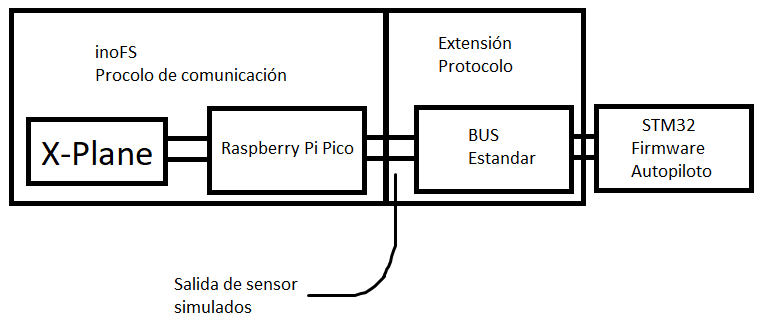
\includegraphics[width=\textwidth]{img/diagrama.png}
\end{frame}

\begin{frame}{Protocolo de comunicación}
	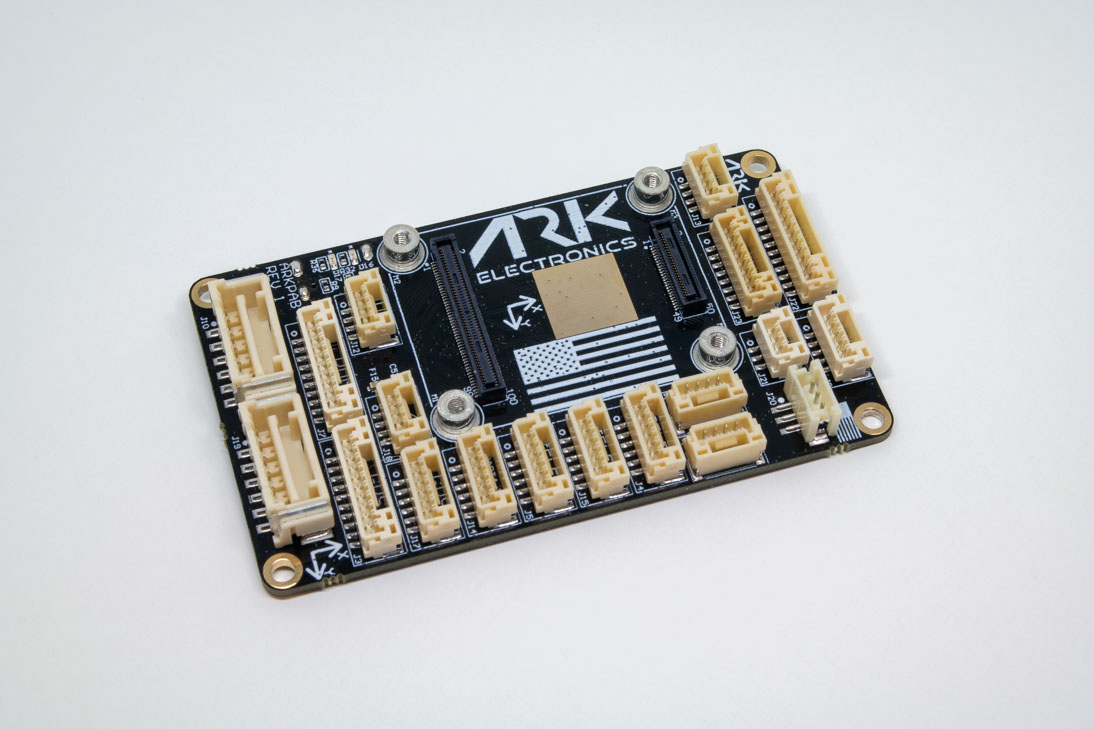
\includegraphics[height=\textheight]{img/bus.jpg}
\end{frame}

\begin{frame}
	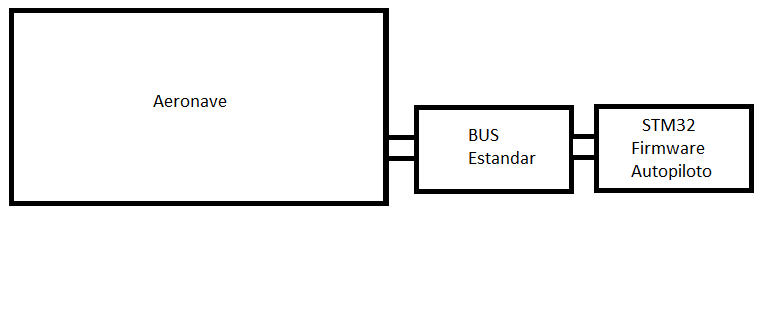
\includegraphics[width=\textwidth]{img/diagrama2.png}
\end{frame}

\subsection{Análisis en simulador}

\begin{frame}

\end{frame}

\end{document}